\section{Странные вещи}

\subsection{Тождество для д...а}

\[
	f(x)\delta(x - x_0) + [F(x) - F(x_0)] \delta'(x - x_0) = 0, \qquad F(x) = \int f(x) dx
\]

\textit{Док-во:}

Продифференцируем тождество:
\[
	F(x) \delta(x - x_0) = F(x_0) \delta(x - x_0)
\]
Просто, не правда ли? В чём подвох? При представлении $\delta$-функции в форме гауссовского предела доказательство упирается в весьма необычные трудности. В частности требуется доказать следующее равенство:
\[
	\lim\limits_{a \to 0} \frac{1}{a}\left(1 - 2 \frac{(x - x_0)^2}{a^2}\right) e^{- \cfrac{(x - x_0)^2}{a^2}} = \lim\limits_{a \to 0} \frac{1}{a} e^{- \cfrac{(x - x_0)^2}{a^2}}
\]
И вот вопрос: как это сделать строго? Казалось бы, что сложного, рассмотрим два случая $x = x_0$ и $x \ne x_0$, равенство выполняется? - Да! Но мне это доказательство не даёт покоя. Кажется, что я что-то упускаю. Тем более, что из тождества следует:
\[
	\delta'(x -x_0) = \frac{1}{x_0 - x} \delta(x -x_0)
\]

\subsection{Ещё одно странное тождество}

\[
	(f(x) \eta(x - a))''_{xx} = f''(x) \eta(x - a) + f'(a) \delta(x - a) + f(a) \delta'(x - a)
\]

\textit{Док-во:}

Снова всё тривиально:
\[
	(f(x) \eta(x - a))''_{xx} = (f'(x) \eta(x - a) + f'(x) \delta(x - a))'_x = (f'(x) \eta(x - a) + f'(a) \delta(x - a))'_x =
	f''(x) \eta(x - a) + f'(a) \delta(x - a) + f(a) \delta'(x - a)
\]

\subsection{Функция отличная от нуля в одной единственной точке}

\[
	f(x) = 2A\eta(-|x-a|) = \begin{cases}
	A, & x = a\\
	0, & x\ne a
	\end{cases}
\]
Наибольший интерес представляет её производная:
\[
	f'(x) = -2A\delta(-|x-a|)\sign(x -a) = 0
\]
Не правда ли замечательно! Теперь решение уравнения:
\[
	y' = 0,\qquad y(0) = y_0
\]
будет выглядеть так:
\[
	y = y_0+\sum\limits_{i, a_i \ne 0} 2 C_i \eta(-|x-a_i|)
\]
То есть в классе функций с разрывами решений бесконечно много! 

Как мне подсказал Antony я вообще говоря не прав, так как здесь имеет место неопределённость вида $\infty\times 0$. Представление в форме предела последовательности для $\delta-$функции, приводит тем не менее к результатам изложенным выше, но при одном дополнительном условии, что пределы можно менять местами, что скорее всего также неправильно. Ещё один способ мог бы быть связан с представлением решения в форме предела:
\[
	\lim\limits_{b \to 0} \eta(x - a - b) - \eta(x - a)
\]
Но как следует из определения $\eta-$функции это тождественно 0. И вопрос о правильности полученных результатов остаётся открытым. Вдогонку к данной проблеме можно рассмотреть следующее интересное тождество:
\[
	\sign^2(x) = |\sign(x)|
\]
Продифференцируем его:
\[
	4 \sign(x) \delta(x) = \sign(\sign(x)) 2\delta(x) = 2 \sign(x) \delta(x) 
\]
Если бы можно было сократить всё лишнее было бы:
\[
	4 = 2
\]
Но к счастью сократить ничего нельзя. Однако, отсюда следует:
\[
	 2 \sign(x) \delta(x) = 0
\]

\subsection{Функция для вычисления площади пересечения треугольника с полуплоскостью}

Рассмотрим треугольник, один из катетов, которого лежит на оси абсцисс, другой параллелен оси ординат и прямую, параллельную оси ординат, делящую плоскость на две полуплоскости, как показано на рисунке:
\begin{center}
	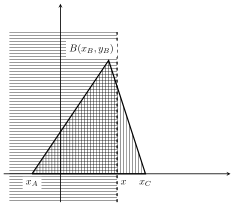
\includegraphics{images/png/triangle_func.png}
	%\usetikzlibrary{patterns}
\begin{tikzpicture}

\draw[thick,-stealth]  (0,-1) -- (0,6);
\draw[thick,-stealth] (-2,0) -- (6,0);
\draw[very thick, pattern=vertical lines] (-1,0) -- (1.7, 4) -- (3,0) -- (-1, 0);
\draw[very thick, dashed] (2, -1) -- (2, 5);
\path[pattern=horizontal lines] (2, -1) rectangle (-1.8, 5);

\node[below, fill = white] at (-1,-0.1) {$x_A$};
\node[above, fill = white] at (1.1,4.1) {$B(x_B, y_B)$};
\node[below] at (3,-0.1) {$x_C$};
\node[below right] at (2,-0.1) {$x$};

\end{tikzpicture}
\end{center}
Площадь области с двойной штриховкой:
\[
	S_+(x, x_A, x_B, x_C, y_B) = 
	\begin{cases}
	0, & x < x_A; \\
	\frac{1}{2} y_B \frac{(x - x_A)^2}{x_B - x_A}, & x_A < x < x_B; \\
	\frac{1}{2} y_B \left[(x_B - x_A) + \frac{2 x_C - x - x_B}{x_C - x_B} (x - x_B)\right] , & x_B < x < x_C; \\
	\frac{1}{2} y_B (x_C - x_A), & x_C < x.
	\end{cases}
\]
Другая полуплоскость, даёт область с одинарной штриховкой:
\[
S_-(x, x_A, x_B, x_C, y_B) = 
\begin{cases}
\frac{1}{2} y_B (x_C - x_A), & x < x_A; \\
\frac{1}{2} y_B \left[(x_C - x_B) + \frac{x_B + x - 2 x_A}{x_B - x_A} (x_B - x)\right], & x_A < x < x_B; \\
\frac{1}{2} y_B \frac{(x_C - x)^2}{x_C - x_B} , & x_B < x < x_C; \\
0, & x_C < x.
\end{cases}
\]
Первую из этих функций можно представить в виде:
\[
	\begin{aligned}
	& S_+(x, x_A, x_B, x_C, y_B) =  
	\frac{1}{2} y_B \frac{(x - x_A)^2}{x_B - x_A} \eta(x - x_A) \eta(x_B - x)  + \\ & +
	\frac{1}{2} y_B \left[(x_B - x_A) + \frac{2 x_C - x - x_B}{x_C - x_B} (x - x_B)\right] \eta(x - x_B) \eta(x_C - x) +
	\frac{1}{2} y_B (x_C - x_A) \eta(x - x_C)
	\end{aligned}
\]
Здесь следует отметить, что представление возможно только если $x_A < x_B < x_C$. Именно для этого случая записаны все выражения выше.